
*%!TEX program = xelatex
*\usepackage[UTF8]{ctex}
\documentclass[11pt]{article}

    
    \usepackage[T1]{fontenc}
    % Nicer default font (+ math font) than Computer Modern for most use cases
    \usepackage{mathpazo}

    % Basic figure setup, for now with no caption control since it's done
    % automatically by Pandoc (which extracts ![](path) syntax from Markdown).
    \usepackage{graphicx}
    % We will generate all images so they have a width \maxwidth. This means
    % that they will get their normal width if they fit onto the page, but
    % are scaled down if they would overflow the margins.
    \makeatletter
    \def\maxwidth{\ifdim\Gin@nat@width>\linewidth\linewidth
    \else\Gin@nat@width\fi}
    \makeatother
    \let\Oldincludegraphics\includegraphics
    % Set max figure width to be 80% of text width, for now hardcoded.
    \renewcommand{\includegraphics}[1]{\Oldincludegraphics[width=.8\maxwidth]{#1}}
    % Ensure that by default, figures have no caption (until we provide a
    % proper Figure object with a Caption API and a way to capture that
    % in the conversion process - todo).
    \usepackage{caption}
    \DeclareCaptionLabelFormat{nolabel}{}
    \captionsetup{labelformat=nolabel}

    \usepackage{adjustbox} % Used to constrain images to a maximum size 
    \usepackage{xcolor} % Allow colors to be defined
    \usepackage{enumerate} % Needed for markdown enumerations to work
    \usepackage{geometry} % Used to adjust the document margins
    \usepackage{amsmath} % Equations
    \usepackage{amssymb} % Equations
    \usepackage{textcomp} % defines textquotesingle
    % Hack from http://tex.stackexchange.com/a/47451/13684:
    \AtBeginDocument{%
        \def\PYZsq{\textquotesingle}% Upright quotes in Pygmentized code
    }
    \usepackage{upquote} % Upright quotes for verbatim code
    \usepackage{eurosym} % defines \euro
    \usepackage[mathletters]{ucs} % Extended unicode (utf-8) support
    \usepackage[utf8x]{inputenc} % Allow utf-8 characters in the tex document
    \usepackage{fancyvrb} % verbatim replacement that allows latex
    \usepackage{grffile} % extends the file name processing of package graphics 
                         % to support a larger range 
    % The hyperref package gives us a pdf with properly built
    % internal navigation ('pdf bookmarks' for the table of contents,
    % internal cross-reference links, web links for URLs, etc.)
    \usepackage{hyperref}
    \usepackage{longtable} % longtable support required by pandoc >1.10
    \usepackage{booktabs}  % table support for pandoc > 1.12.2
    \usepackage[inline]{enumitem} % IRkernel/repr support (it uses the enumerate* environment)
    \usepackage[normalem]{ulem} % ulem is needed to support strikethroughs (\sout)
                                % normalem makes italics be italics, not underlines
    

    
    
    % Colors for the hyperref package
    \definecolor{urlcolor}{rgb}{0,.145,.698}
    \definecolor{linkcolor}{rgb}{.71,0.21,0.01}
    \definecolor{citecolor}{rgb}{.12,.54,.11}

    % ANSI colors
    \definecolor{ansi-black}{HTML}{3E424D}
    \definecolor{ansi-black-intense}{HTML}{282C36}
    \definecolor{ansi-red}{HTML}{E75C58}
    \definecolor{ansi-red-intense}{HTML}{B22B31}
    \definecolor{ansi-green}{HTML}{00A250}
    \definecolor{ansi-green-intense}{HTML}{007427}
    \definecolor{ansi-yellow}{HTML}{DDB62B}
    \definecolor{ansi-yellow-intense}{HTML}{B27D12}
    \definecolor{ansi-blue}{HTML}{208FFB}
    \definecolor{ansi-blue-intense}{HTML}{0065CA}
    \definecolor{ansi-magenta}{HTML}{D160C4}
    \definecolor{ansi-magenta-intense}{HTML}{A03196}
    \definecolor{ansi-cyan}{HTML}{60C6C8}
    \definecolor{ansi-cyan-intense}{HTML}{258F8F}
    \definecolor{ansi-white}{HTML}{C5C1B4}
    \definecolor{ansi-white-intense}{HTML}{A1A6B2}

    % commands and environments needed by pandoc snippets
    % extracted from the output of `pandoc -s`
    \providecommand{\tightlist}{%
      \setlength{\itemsep}{0pt}\setlength{\parskip}{0pt}}
    \DefineVerbatimEnvironment{Highlighting}{Verbatim}{commandchars=\\\{\}}
    % Add ',fontsize=\small' for more characters per line
    \newenvironment{Shaded}{}{}
    \newcommand{\KeywordTok}[1]{\textcolor[rgb]{0.00,0.44,0.13}{\textbf{{#1}}}}
    \newcommand{\DataTypeTok}[1]{\textcolor[rgb]{0.56,0.13,0.00}{{#1}}}
    \newcommand{\DecValTok}[1]{\textcolor[rgb]{0.25,0.63,0.44}{{#1}}}
    \newcommand{\BaseNTok}[1]{\textcolor[rgb]{0.25,0.63,0.44}{{#1}}}
    \newcommand{\FloatTok}[1]{\textcolor[rgb]{0.25,0.63,0.44}{{#1}}}
    \newcommand{\CharTok}[1]{\textcolor[rgb]{0.25,0.44,0.63}{{#1}}}
    \newcommand{\StringTok}[1]{\textcolor[rgb]{0.25,0.44,0.63}{{#1}}}
    \newcommand{\CommentTok}[1]{\textcolor[rgb]{0.38,0.63,0.69}{\textit{{#1}}}}
    \newcommand{\OtherTok}[1]{\textcolor[rgb]{0.00,0.44,0.13}{{#1}}}
    \newcommand{\AlertTok}[1]{\textcolor[rgb]{1.00,0.00,0.00}{\textbf{{#1}}}}
    \newcommand{\FunctionTok}[1]{\textcolor[rgb]{0.02,0.16,0.49}{{#1}}}
    \newcommand{\RegionMarkerTok}[1]{{#1}}
    \newcommand{\ErrorTok}[1]{\textcolor[rgb]{1.00,0.00,0.00}{\textbf{{#1}}}}
    \newcommand{\NormalTok}[1]{{#1}}
    
    % Additional commands for more recent versions of Pandoc
    \newcommand{\ConstantTok}[1]{\textcolor[rgb]{0.53,0.00,0.00}{{#1}}}
    \newcommand{\SpecialCharTok}[1]{\textcolor[rgb]{0.25,0.44,0.63}{{#1}}}
    \newcommand{\VerbatimStringTok}[1]{\textcolor[rgb]{0.25,0.44,0.63}{{#1}}}
    \newcommand{\SpecialStringTok}[1]{\textcolor[rgb]{0.73,0.40,0.53}{{#1}}}
    \newcommand{\ImportTok}[1]{{#1}}
    \newcommand{\DocumentationTok}[1]{\textcolor[rgb]{0.73,0.13,0.13}{\textit{{#1}}}}
    \newcommand{\AnnotationTok}[1]{\textcolor[rgb]{0.38,0.63,0.69}{\textbf{\textit{{#1}}}}}
    \newcommand{\CommentVarTok}[1]{\textcolor[rgb]{0.38,0.63,0.69}{\textbf{\textit{{#1}}}}}
    \newcommand{\VariableTok}[1]{\textcolor[rgb]{0.10,0.09,0.49}{{#1}}}
    \newcommand{\ControlFlowTok}[1]{\textcolor[rgb]{0.00,0.44,0.13}{\textbf{{#1}}}}
    \newcommand{\OperatorTok}[1]{\textcolor[rgb]{0.40,0.40,0.40}{{#1}}}
    \newcommand{\BuiltInTok}[1]{{#1}}
    \newcommand{\ExtensionTok}[1]{{#1}}
    \newcommand{\PreprocessorTok}[1]{\textcolor[rgb]{0.74,0.48,0.00}{{#1}}}
    \newcommand{\AttributeTok}[1]{\textcolor[rgb]{0.49,0.56,0.16}{{#1}}}
    \newcommand{\InformationTok}[1]{\textcolor[rgb]{0.38,0.63,0.69}{\textbf{\textit{{#1}}}}}
    \newcommand{\WarningTok}[1]{\textcolor[rgb]{0.38,0.63,0.69}{\textbf{\textit{{#1}}}}}
  
    \begin{titlepage}

\begin{center}


% Upper part of the page  

\textsc{\Large Searching the lost plane MH370 by bayesian method}\\[0.5cm]

    \end{center}
% Title
\HRule \\[0.4cm]


\HRule \\[1.5cm]
\begin{center}
% Author and supervisor
\begin{minipage}{0.4\textwidth}
\begin{flushleft} \large
\emph{Author:}\\
Junjie Liu, Terry 1630005038

Zhifan Gao, Eunice 1630005014 

Yihe, Eliza He 1630005019

\end{flushleft}
\end{minipage}
\end{center}
\vfill
  \begin{center}
    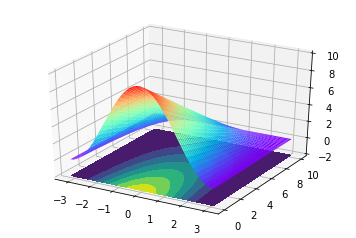
\includegraphics[scale=0.6]{output_3_0.png}
    \end{center}
% Bottom of the page
{\large \today}
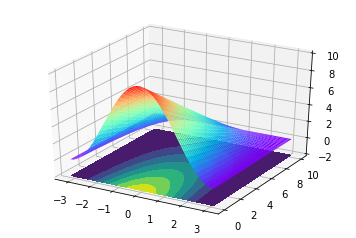
\includegraphics[width=0.15\textwidth]{output_3_0.png}\\[1cm]
\end{center}

\end{titlepage}
    % Define a nice break command that doesn't care if a line doesn't already
    % exist.
    \def\br{\hspace*{\fill} \\* }
    % Math Jax compatability definitions
    \def\gt{>}
    \def\lt{<}
    % Document parameters    
    

    % Pygments definitions
    
\makeatletter
\def\PY@reset{\let\PY@it=\relax \let\PY@bf=\relax%
    \let\PY@ul=\relax \let\PY@tc=\relax%
    \let\PY@bc=\relax \let\PY@ff=\relax}
\def\PY@tok#1{\csname PY@tok@#1\endcsname}
\def\PY@toks#1+{\ifx\relax#1\empty\else%
    \PY@tok{#1}\expandafter\PY@toks\fi}
\def\PY@do#1{\PY@bc{\PY@tc{\PY@ul{%
    \PY@it{\PY@bf{\PY@ff{#1}}}}}}}
\def\PY#1#2{\PY@reset\PY@toks#1+\relax+\PY@do{#2}}

\expandafter\def\csname PY@tok@w\endcsname{\def\PY@tc##1{\textcolor[rgb]{0.73,0.73,0.73}{##1}}}
\expandafter\def\csname PY@tok@c\endcsname{\let\PY@it=\textit\def\PY@tc##1{\textcolor[rgb]{0.25,0.50,0.50}{##1}}}
\expandafter\def\csname PY@tok@cp\endcsname{\def\PY@tc##1{\textcolor[rgb]{0.74,0.48,0.00}{##1}}}
\expandafter\def\csname PY@tok@k\endcsname{\let\PY@bf=\textbf\def\PY@tc##1{\textcolor[rgb]{0.00,0.50,0.00}{##1}}}
\expandafter\def\csname PY@tok@kp\endcsname{\def\PY@tc##1{\textcolor[rgb]{0.00,0.50,0.00}{##1}}}
\expandafter\def\csname PY@tok@kt\endcsname{\def\PY@tc##1{\textcolor[rgb]{0.69,0.00,0.25}{##1}}}
\expandafter\def\csname PY@tok@o\endcsname{\def\PY@tc##1{\textcolor[rgb]{0.40,0.40,0.40}{##1}}}
\expandafter\def\csname PY@tok@ow\endcsname{\let\PY@bf=\textbf\def\PY@tc##1{\textcolor[rgb]{0.67,0.13,1.00}{##1}}}
\expandafter\def\csname PY@tok@nb\endcsname{\def\PY@tc##1{\textcolor[rgb]{0.00,0.50,0.00}{##1}}}
\expandafter\def\csname PY@tok@nf\endcsname{\def\PY@tc##1{\textcolor[rgb]{0.00,0.00,1.00}{##1}}}
\expandafter\def\csname PY@tok@nc\endcsname{\let\PY@bf=\textbf\def\PY@tc##1{\textcolor[rgb]{0.00,0.00,1.00}{##1}}}
\expandafter\def\csname PY@tok@nn\endcsname{\let\PY@bf=\textbf\def\PY@tc##1{\textcolor[rgb]{0.00,0.00,1.00}{##1}}}
\expandafter\def\csname PY@tok@ne\endcsname{\let\PY@bf=\textbf\def\PY@tc##1{\textcolor[rgb]{0.82,0.25,0.23}{##1}}}
\expandafter\def\csname PY@tok@nv\endcsname{\def\PY@tc##1{\textcolor[rgb]{0.10,0.09,0.49}{##1}}}
\expandafter\def\csname PY@tok@no\endcsname{\def\PY@tc##1{\textcolor[rgb]{0.53,0.00,0.00}{##1}}}
\expandafter\def\csname PY@tok@nl\endcsname{\def\PY@tc##1{\textcolor[rgb]{0.63,0.63,0.00}{##1}}}
\expandafter\def\csname PY@tok@ni\endcsname{\let\PY@bf=\textbf\def\PY@tc##1{\textcolor[rgb]{0.60,0.60,0.60}{##1}}}
\expandafter\def\csname PY@tok@na\endcsname{\def\PY@tc##1{\textcolor[rgb]{0.49,0.56,0.16}{##1}}}
\expandafter\def\csname PY@tok@nt\endcsname{\let\PY@bf=\textbf\def\PY@tc##1{\textcolor[rgb]{0.00,0.50,0.00}{##1}}}
\expandafter\def\csname PY@tok@nd\endcsname{\def\PY@tc##1{\textcolor[rgb]{0.67,0.13,1.00}{##1}}}
\expandafter\def\csname PY@tok@s\endcsname{\def\PY@tc##1{\textcolor[rgb]{0.73,0.13,0.13}{##1}}}
\expandafter\def\csname PY@tok@sd\endcsname{\let\PY@it=\textit\def\PY@tc##1{\textcolor[rgb]{0.73,0.13,0.13}{##1}}}
\expandafter\def\csname PY@tok@si\endcsname{\let\PY@bf=\textbf\def\PY@tc##1{\textcolor[rgb]{0.73,0.40,0.53}{##1}}}
\expandafter\def\csname PY@tok@se\endcsname{\let\PY@bf=\textbf\def\PY@tc##1{\textcolor[rgb]{0.73,0.40,0.13}{##1}}}
\expandafter\def\csname PY@tok@sr\endcsname{\def\PY@tc##1{\textcolor[rgb]{0.73,0.40,0.53}{##1}}}
\expandafter\def\csname PY@tok@ss\endcsname{\def\PY@tc##1{\textcolor[rgb]{0.10,0.09,0.49}{##1}}}
\expandafter\def\csname PY@tok@sx\endcsname{\def\PY@tc##1{\textcolor[rgb]{0.00,0.50,0.00}{##1}}}
\expandafter\def\csname PY@tok@m\endcsname{\def\PY@tc##1{\textcolor[rgb]{0.40,0.40,0.40}{##1}}}
\expandafter\def\csname PY@tok@gh\endcsname{\let\PY@bf=\textbf\def\PY@tc##1{\textcolor[rgb]{0.00,0.00,0.50}{##1}}}
\expandafter\def\csname PY@tok@gu\endcsname{\let\PY@bf=\textbf\def\PY@tc##1{\textcolor[rgb]{0.50,0.00,0.50}{##1}}}
\expandafter\def\csname PY@tok@gd\endcsname{\def\PY@tc##1{\textcolor[rgb]{0.63,0.00,0.00}{##1}}}
\expandafter\def\csname PY@tok@gi\endcsname{\def\PY@tc##1{\textcolor[rgb]{0.00,0.63,0.00}{##1}}}
\expandafter\def\csname PY@tok@gr\endcsname{\def\PY@tc##1{\textcolor[rgb]{1.00,0.00,0.00}{##1}}}
\expandafter\def\csname PY@tok@ge\endcsname{\let\PY@it=\textit}
\expandafter\def\csname PY@tok@gs\endcsname{\let\PY@bf=\textbf}
\expandafter\def\csname PY@tok@gp\endcsname{\let\PY@bf=\textbf\def\PY@tc##1{\textcolor[rgb]{0.00,0.00,0.50}{##1}}}
\expandafter\def\csname PY@tok@go\endcsname{\def\PY@tc##1{\textcolor[rgb]{0.53,0.53,0.53}{##1}}}
\expandafter\def\csname PY@tok@gt\endcsname{\def\PY@tc##1{\textcolor[rgb]{0.00,0.27,0.87}{##1}}}
\expandafter\def\csname PY@tok@err\endcsname{\def\PY@bc##1{\setlength{\fboxsep}{0pt}\fcolorbox[rgb]{1.00,0.00,0.00}{1,1,1}{\strut ##1}}}
\expandafter\def\csname PY@tok@kc\endcsname{\let\PY@bf=\textbf\def\PY@tc##1{\textcolor[rgb]{0.00,0.50,0.00}{##1}}}
\expandafter\def\csname PY@tok@kd\endcsname{\let\PY@bf=\textbf\def\PY@tc##1{\textcolor[rgb]{0.00,0.50,0.00}{##1}}}
\expandafter\def\csname PY@tok@kn\endcsname{\let\PY@bf=\textbf\def\PY@tc##1{\textcolor[rgb]{0.00,0.50,0.00}{##1}}}
\expandafter\def\csname PY@tok@kr\endcsname{\let\PY@bf=\textbf\def\PY@tc##1{\textcolor[rgb]{0.00,0.50,0.00}{##1}}}
\expandafter\def\csname PY@tok@bp\endcsname{\def\PY@tc##1{\textcolor[rgb]{0.00,0.50,0.00}{##1}}}
\expandafter\def\csname PY@tok@fm\endcsname{\def\PY@tc##1{\textcolor[rgb]{0.00,0.00,1.00}{##1}}}
\expandafter\def\csname PY@tok@vc\endcsname{\def\PY@tc##1{\textcolor[rgb]{0.10,0.09,0.49}{##1}}}
\expandafter\def\csname PY@tok@vg\endcsname{\def\PY@tc##1{\textcolor[rgb]{0.10,0.09,0.49}{##1}}}
\expandafter\def\csname PY@tok@vi\endcsname{\def\PY@tc##1{\textcolor[rgb]{0.10,0.09,0.49}{##1}}}
\expandafter\def\csname PY@tok@vm\endcsname{\def\PY@tc##1{\textcolor[rgb]{0.10,0.09,0.49}{##1}}}
\expandafter\def\csname PY@tok@sa\endcsname{\def\PY@tc##1{\textcolor[rgb]{0.73,0.13,0.13}{##1}}}
\expandafter\def\csname PY@tok@sb\endcsname{\def\PY@tc##1{\textcolor[rgb]{0.73,0.13,0.13}{##1}}}
\expandafter\def\csname PY@tok@sc\endcsname{\def\PY@tc##1{\textcolor[rgb]{0.73,0.13,0.13}{##1}}}
\expandafter\def\csname PY@tok@dl\endcsname{\def\PY@tc##1{\textcolor[rgb]{0.73,0.13,0.13}{##1}}}
\expandafter\def\csname PY@tok@s2\endcsname{\def\PY@tc##1{\textcolor[rgb]{0.73,0.13,0.13}{##1}}}
\expandafter\def\csname PY@tok@sh\endcsname{\def\PY@tc##1{\textcolor[rgb]{0.73,0.13,0.13}{##1}}}
\expandafter\def\csname PY@tok@s1\endcsname{\def\PY@tc##1{\textcolor[rgb]{0.73,0.13,0.13}{##1}}}
\expandafter\def\csname PY@tok@mb\endcsname{\def\PY@tc##1{\textcolor[rgb]{0.40,0.40,0.40}{##1}}}
\expandafter\def\csname PY@tok@mf\endcsname{\def\PY@tc##1{\textcolor[rgb]{0.40,0.40,0.40}{##1}}}
\expandafter\def\csname PY@tok@mh\endcsname{\def\PY@tc##1{\textcolor[rgb]{0.40,0.40,0.40}{##1}}}
\expandafter\def\csname PY@tok@mi\endcsname{\def\PY@tc##1{\textcolor[rgb]{0.40,0.40,0.40}{##1}}}
\expandafter\def\csname PY@tok@il\endcsname{\def\PY@tc##1{\textcolor[rgb]{0.40,0.40,0.40}{##1}}}
\expandafter\def\csname PY@tok@mo\endcsname{\def\PY@tc##1{\textcolor[rgb]{0.40,0.40,0.40}{##1}}}
\expandafter\def\csname PY@tok@ch\endcsname{\let\PY@it=\textit\def\PY@tc##1{\textcolor[rgb]{0.25,0.50,0.50}{##1}}}
\expandafter\def\csname PY@tok@cm\endcsname{\let\PY@it=\textit\def\PY@tc##1{\textcolor[rgb]{0.25,0.50,0.50}{##1}}}
\expandafter\def\csname PY@tok@cpf\endcsname{\let\PY@it=\textit\def\PY@tc##1{\textcolor[rgb]{0.25,0.50,0.50}{##1}}}
\expandafter\def\csname PY@tok@c1\endcsname{\let\PY@it=\textit\def\PY@tc##1{\textcolor[rgb]{0.25,0.50,0.50}{##1}}}
\expandafter\def\csname PY@tok@cs\endcsname{\let\PY@it=\textit\def\PY@tc##1{\textcolor[rgb]{0.25,0.50,0.50}{##1}}}

\def\PYZbs{\char`\\}
\def\PYZus{\char`\_}
\def\PYZob{\char`\{}
\def\PYZcb{\char`\}}
\def\PYZca{\char`\^}
\def\PYZam{\char`\&}
\def\PYZlt{\char`\<}
\def\PYZgt{\char`\>}
\def\PYZsh{\char`\#}
\def\PYZpc{\char`\%}
\def\PYZdl{\char`\$}
\def\PYZhy{\char`\-}
\def\PYZsq{\char`\'}
\def\PYZdq{\char`\"}
\def\PYZti{\char`\~}
% for compatibility with earlier versions
\def\PYZat{@}
\def\PYZlb{[}
\def\PYZrb{]}
\makeatother


    % Exact colors from NB
    \definecolor{incolor}{rgb}{0.0, 0.0, 0.5}
    \definecolor{outcolor}{rgb}{0.545, 0.0, 0.0}



    
    % Prevent overflowing lines due to hard-to-break entities
    \sloppy 
    % Setup hyperref package
    \hypersetup{
      breaklinks=true,  % so long urls are correctly broken across lines
      colorlinks=true,
      urlcolor=urlcolor,
      linkcolor=linkcolor,
      citecolor=citecolor,
      }
    % Slightly bigger margins than the latex defaults
    
    \geometry{verbose,tmargin=1in,bmargin=1in,lmargin=1in,rmargin=1in}
    
    

    \begin{document}
    
    
    \maketitle
    
 \tableofcontents   
\hypertarget{Introduction}{%
\section{Introduction}\label{Introduction}}
 \indent There was a very serious and tragic air crash in 2014. The MH370 flight planned from Kuala Lumpur to Beijing lost its signal about 40 minutes after takeoff and eventually failed to reach the end of the flight to Beijing. Many countries in the vicinity of the missing plane has been searching for the first time, but no sign of the plane has been found. Until four years later, MH370 is still a mystery, still no traces of the aircraft found.There are many reasons for not finding the plane that crashed. One of the important reasons for this is that the search area is inaccurate, which means that the location and search scheme of the wrecked aircraft may greatly affect the efficiency of the search. So we considered the process of the plane crash as a physical model, and when the plane crashed into the ocean,we try to use Bayesian search to the plane.\\
    
    \hypertarget{analysis-of-the-problem}{%
\section{Analysis of the Problem}\label{analysis-of-the-problem}}

For finding a missing aircraft, we can split it into two part: First, we
have to predict the descending route of the aircraft and the searching
area; Then, we have to calculate the probability of each area. Also,
after some discussion, we came to the conclusion that we should consider
the possibility of turning during gliding and taxiing. Each area does
not have the some probability, we use the bayesian networks model. This
model can represent the probabilistic relationship between the
probability and the sliding distance and the deviation from the
predetermined trajectory.

\tableofcontents
\hypertarget{Assumption}{%
\section{Assumption}\label{Assumption}}
\hypertarget{Wind and ocean currents}{%
\subsection{Wind and ocean currents}\label{Wind and ocean currents}}
For a whole range of search areas, the effect of ocean currents is weak, and we will not consider the impact of ocean currents on the displacement of falling aircraft in the sea.\\
And also no considering of the wind in the course of the plane's descent.\\
\hypertarget{Plane crash process}{%
\subsection{Plane crash process}\label{Plane crash process}}
\hypertarget{Assumption of aircraft falling outside conditions}{%
\subsubsection{Assumption of aircraft falling outside conditions}\label{Assumption of aircraft falling outside conditions}}
Assuming the plane doesn't disintegrate during the falling.\\
    The last time signal of MH370 was at sea, according to MH370 's flight route, we assumed that the plane would crash into the ocean rather than land.\\
    After the aircraft engine failure, the fall direction and velocity direction are the same, no deviation in the direction.\\
\hypertarget{Simple calculation of the falling position of aircraft}{%
\subsubsection{Simple calculation of the falling position of aircraft}\label{Simple calculation of the falling position of aircraft}}
the following symbol are appear in our equations to solve the problem.\\
\begin{tabular}{cc}
$F$&Air Force\\
$F_1$&Flight lift\\
$f$&Flight resistance\\
$Mg$& Weight of plane\\
$H$& Altitude\\
$\rho_0$& Standard state, sea level atmospheric density\\
$\rho_H$& When altitude is\ $ H$, sea level atmospheric density\\
$\rho$& Average of atmospheric density\\
$C_1$& Lift coefficient\\
$C_f$& Resistance coefficient\\
$S_1$& Aircraft Wing Area\\
$S_2$& Area of force to be affected\\
$a_x$&When falling, horizontal acceleration\\
$a_y$&When falling, vertical acceleration\\
$v$&When falling, velocity\\
$v_x$&When falling, horizontal velocity\\
$v_y$&When falling, vertical velocity\\
$t$&The time when the plane crashed to the sea\\
$x$&When falling, the horizontal axis\\
$y$&When falling, the vertical axis\\
\end{tabular}
\\\\
we assume that, after the aircraft's engine failed, the fuel ran out and the plane started to fall without power but it still has a speed. and then, we have a force analysis of aircraft. The plane will be subjected to the force of gravity(Mg) and air(F).The force of air on an aircraft can be broken down into vertical lift and horizontal resistance.\cite{焦晓君2015一种落水失联飞机的搜寻方案} As shown in Figure.\\
%figure 1
\begin{center}
    \adjustimage{max size={0.3\linewidth}{0.3\paperheight}}{606.png}
    \end{center}
From the formula for calculating the lift of aircraft, we can draw:\\
\[F_1=\frac{1}{2}C_1\rho v^2 S_1\] 
From the formula for calculating the resistance of aircraft, we can draw:\\
\[f=\frac{1}{2}C_f\rho v^2 S_2\] 

Because atmospheric density varies according to altitude.After querying the relevant data, we obtained the formula between altitude and atmospheric density.\\

\[\rho_H=\rho_0(1-2.25577\times 10^{-5}H)^{4.25588}\] 
since the last time the plane sent a signal, the flight altitude was 35000 feet (10668m)\\
so we assume $H=10000m$, and calculate $\rho_H=0.4007 \ kg/m^3$\\
then we can draw the graph of $\rho_H$\\
%figure 2
\begin{center}
    \adjustimage{max size={0.5\linewidth}{0.5\paperheight}}{603.png}
    \end{center}
from this graph, we can consider it to a linear model, and then find the average $\rho $as the atmospheric density we use in this problem.\\
then we can get:\\

\[\rho=\frac{1.225+0.4007}{2}=0.8129 \approx 0.8\ kg/m^3\]
Next we'll build a coordinate system\\
The flight direction of the plane is $X-axis$;\  Vertical direction is $Y-axis$\\
Next, we can decompose the acceleration according to the force direction.\\
Finally, we have following equations:\\
\[f=Ma_x\]
\[Mg-F_1=Ma_y\] 
according to the formula for calculating velocity and acceleration,we can get:\\

\[v_x=\frac{dx}{dt}\]


\[a_x=\frac{d^2x}{dt^2}\]
in the same way, \\

\[x=v_xt\]

\[a_y=\frac{d^2y}{dt^2}\]
Finally, we can get:\\

\[\frac{1}{2}\rho( \frac{dx}{dt})^2 S_1=M\frac{d^2x}{dt^2}\] 

\[\frac{1}{2}\rho( \frac{dy}{dt})^2 S_2=Mg-M\frac{d^2y}{dt^2}\]
\\\\
we can use matlab to solve these two differential equations.\\
According to the plane of the MH370 flight, the information of the Boeing 777-200ER, we assume that $S_1=400m^2$; $S_2=300m^2$; $C_1=1.5$; $C_f=0.09$; $M=200000kg$;\\
$y(0)=10000m$; $x(0)=0$; $y'(0)=0$; $x'(0)=250m/s$\cite{Jenkinson1999Civil}\\
\\
then we can get a graph of Plane Fall trajectory:\\
%figure 3
\begin{center}
    \adjustimage{max size={0.5\linewidth}{0.5\paperheight}}{607.png}
    \end{center}
and also we can get the time (t) of the plane from losing power to falling sea is\ $ t=117.0485s$\\
$x=17553m$, so the point that the plane fall into the sea is (17553,0)\\

\tableofcontents

\hypertarget{Bayesian Method}{%
\section{Bayesian Method}\label{Bayesian method}}
\hypertarget{Comparison of search methods}{%
\subsection{Comparison of Search Methods}\label{Comparison of search methods}}
In many search methods, we first consider the parallel sweep search method. If we have sufficient resources and can search without considering any time cost, a parallel sweep search method is available to find the crashed aircraft. But the rescue time is valuable, the scope is broad, the sea terrain is complex, so the use of this method of search efficiency will be very low, it is likely to miss the best rescue time. So we hope to be able to search and rescue from the place with the highest probability of plane crash. The Bayesian search method can calculate the probability of finding a crashed plane in comparison to the parallel sweep search method. According to the probability, we can search from high probability to low, in order to maximize the rescue time.\\
\begin{center}
    \adjustimage{max size={0.4\linewidth}{0.4\paperheight}}{601.png}
    \end{center}
\hypertarget{Bayesian Search method}{%
\subsection{Bayesian Search Method}\label{Bayesian search method}}
We give a bounded the search area and sperated them some disjoint
sub-areas. Each sub-areas has it own specific probabilty of cataining
the aircarft or its wreckage. This probability is also the initial
probability. We also use Bayes' Theorem to get the probability of
finding the wreckage. The formula of Bayes's Theorem is as follows:
\[P(A|B) = \frac{P(A \cap B)}{P(B)} = \frac{P(A)\cap P(B)}{\sum P(A)\bullet P(B_i)} \]
The posteriori probability is ``finding hte plane'' and the initial
probability is ``the plane or its wrckage is in this sub-areas. The
theorem also has another explanation: If we get the \(p\) as the
probability that a sub-area is contain the plane, and if the plane is
successfully found in this sub-area, we give it a new probability \(q\).
If we did not found the plane, we can use Bayes'theorem to update \(p\)
to \(p'\): \[p' = \frac{p(1-q)}{(1-p)+p(1-q)}\] For each sub-area, we
assume that the probability before the searching is \(r\), the prior
probability). If this sub-area is been searched and the aircraft is not
found, the probabilities of other sub-area will be increased and we
assume the probability is \(r'\)(the posterior probaility). We can get a
new formula: \[r' = \frac{r}{1-pq} > r\] Through this formula, we can
continually update our modal and the probabilties of the remaining
sub-areas. What's more, this formula also can renomalize the probability
distribution, which means we have 100\% confidence that the aircraft is
in the sub-areas.\\
    \hypertarget{Probability of Containing}{%
\section{Probability of Containing}\label{Probability of Containing}}
Before we use the Bayes Search Method, we must first ensure which area the downed plane could be. That is the 'p' in the function of Bayes Search Method. We need to get ratio between each small area and by this ratio a probability density function can be get. By the same time there is not only one possibility  for the plane falling down. So we need to consider about all possibilities and calculate the weight of each possibility, then we can get the final probability that the plane is in that area. Then we can use Bayes Search Method too solve the problem.
\hypertarget{Two Dropping Model}{%
\subsection{Two Dropping Model}\label{Two Dropping Model}}
From our assumptions, the downed plane we are searching for cannot transmit signals.  So we only can rely on the last signal from the plane that we received. Because the last contact of Malaysia Airlines Flight 370 was when the plane left the range of Malaysian Military radar while over the Andaman Sea. From the last radar detection we can get many important information about the downed plane, such as its direction, altitude, speed, and so on at last contact. From the last radar detection and those information we can form two generally reasonable guesses about how the plane behaved in the time immediately following. Then we will give you the two guesses in different condition as follow.
\hypertarget{Model 1: Flying Model}{%
\subsubsection{Model 1: Flying Model}\label{ Model 1: Flying Model}}
The first model we consider about only the signals can't be received that is the plan still can fly. This model is about the time after the plane can't find by radio, it can fly until the fuel runs out of. That is the time and place it begins to fall into the ocean. Using the information such as, altitude, speed, direction, that we get from the final radar detection, we can compute how far the plane can fly after we can't receive the  signals before running out of fuel. Let the longest of the distance it can fly as D. As the Flying Model consider about the largest probability is the air plan uses all of its fuel to fly. Therefore we can assume that the largest probability of the  distance it flies after can't be detected by radio is the probability of D. For the direction it flies after can't be detected by radio, the most likely one is to fly straight forward. Then we can get the probability of both sides is symmetry by the trajectory which fly straight forward.\\
Let $p_1$ be the un-normalized formula for the Flying Model. Then we can get
\[p_1=r*cos^2(\theta/2), ~ ~ ~ ~ r\in[0,D], ~ ~ ~ ~ \theta\in[-\pi,\pi]\]
So when r is 0, the downed plane begins to fall at the point where we lost contact with the plane, and for any $\theta$, $p_1=0$. When r is D, that is the point the plane begins to fall is D  away from where it can't detecte by radio, we can get the largest $p_1$. As the angle $\theta$ farther away from zero, the $p_1$ become smaller. We show this probability in pictures.\\
the red part in the picture is the area where have the highest probability , and purple part is the area where has the lowest probability. \\
\begin{center}
    \adjustimage{max size={0.5\linewidth}{0.5\paperheight}}{111.png}
    \end{center}
\hypertarget{Model 2: Falling Model}{%
\subsubsection{Model 2: Falling Model}\label{Model 2: Falling Model}}
Then we will consider the second case. When the signal station receives the final signal from the plane, the plane has broken down, it may be directly down, as we assume in the 2nd hypothesis, or it is possible to move forward briefly after the fall.\\
So in the second case, the value of R will be between the displacement x of the plane falling directly and the maximum displacement $D $of the plane. Next we consider the probability that there may be any aircraft remains in the area where the plane crashed. We use the following formula to calculate.\\
\[p_2=(D-r)*cos^2(\theta/2), ~ ~ ~ ~ r\in[x,D], ~ ~ ~ ~ \theta\in[-\pi,\pi]\]
When r takes a value of x, the direction of descent may not be fixed if it has a direct drop of the horizontal initial velocity, but once the plane breaks down and begins to fall, the direction cannot be adjusted again. \\We still use color to represent the probability of a plane falling.\\
\begin{center}
    \adjustimage{max size={0.5\linewidth}{0.5\paperheight}}{222.png}
    \end{center}
the red part in the picture is the area where have the highest probability , and purple part is the area where has the lowest probability. \\
\hypertarget{the final distribution of probability}{%
\subsection{The Final Distribution of Probability}\label{The Final Distribution of Probability}}
Based on the two models we discussed above, flying model and failing model.  we get different probability distributions. We want to combine the two patterns in one way . So we will assign different weights to the two models according to the actual situation, to get a final probability distribution.\\
this is the following formula:\\
{$P=w_1p_1+w_2p_2$}\\
and $w_1$ and $w_2$ are the appropriate weight, which means:\\
{$0 \leq w_1, w_2 \leq 1$ and $w_1+w_2=1$}\\
then, what we need to consider about how to calculate the $w_1$ and $w_2$\\
\hypertarget{Calculate the Weight}{%
\subsection{Calculate the Weight}\label{Calculate the Weight}}
we assume that there are two variables, one is H', the altitude of the aircraft in general, H, the altitude when the aircraft last received the signal.\\
If H is a relatively number close to 0, then we can assume that the plane has started to crash, then this is a tendency to fall into the model. If H is a value close to the general flight value H ', we can assume that the plane is not broken at that time and tends to be the first flight model we discuss.\\
then we have a rate:\\
\[w_1=\frac{H}{H'}\]
if $H$ close to $H'$, the rate $w_1 $will close to 1, than means we tend to choose the flying model.\\
if $H $close to 0, the rate $w_1$ will close to 0, than means we not tend to choose the flying model.\\
in this way, we can show the weight in the equation.\\
here we can have the graph of final distribution of probability\\
\begin{center}
    \adjustimage{max size={0.5\linewidth}{0.5\paperheight}}{333.png}
    \end{center}

    \hypertarget{finding Model}{%
\section{Finding Model}\label{finding Model}}
\hypertarget{introduction}{%
\subsection{ Introduction}\label{ Introduction}}
In the two model, we can see that we split the ocean into a square lattice, so the search only needs to search every lattice and starting the search from the maximum probability grid.\\
In our model, the discretization of the search area is carried out under square, and the probability distribution of the location of the downed plane can be ensure with a high probability in an area. In this case, the probability of the downed plane is found in any square is approximately equal.In the 5 Probability of Containing we consider about where the plane may drop, and in 6 Finding Model we consider about find. There is a correlation probability of detecting the downed plane for each search container. 
\hypertarget{ Find the 'q'}{%
\subsection{  Find the 'q'}\label{  Find the 'q'}}
Let $p(z)$ be the probability of finding the downed plane between the search equipment is z.\\
Let K be the width of each square\\
\begin{center}
    \adjustimage{max size={0.5\linewidth}{0.5\paperheight}}{555.png}
    \end{center}
Let our search go though along a path with the length $L$ divided into $n$ parts and we can get the length of each part is $L/n$.We can make an assumption that the probability of the downed plane follows the uniform distributed. We can fond that the area between the curve p(x) and axis equal to 1. And the probability of width K is also 1.For each square with search width K, search length $L/n$,(K is also the probability that we can find the airplane in the square), the probability of the downed plane can be find in the square is 
\[KL/n\]
For n square, the probability of we can not find the downed plane is
\[
(1-KL/n)^n
\]
Therefore, the probability of we can find the downed plane can be find in n squares is q
\[
q=1-(1-KL/n)^n
\]



    \hypertarget{improving-the-model}{%
\section{Improving the Model}\label{inproving-the-model}}

In fact, there are many reasons why it is difficult to find out after
the plane is lost its communication. So it turns out that looking for
the missing plane is actually associated with a lot of variables. In our
model, it's one of the simplified models that doesn't take a lot of
reality into account. The plane crashed into the sea and for some reason
could not be located for long. “Perhaps the most famous case was MH370
Malaysia airlines flight and air France flight 447. Although MH370
flights are still missing, flight 447 in the second years after the
crash happened founded by a team.”\cite{chen2012fvcom} \cite{} the method they used is called:
recursive tracking \#\# Recursive Tracking The team is developed and
worked on recursive tracking. In short, the method is says: the planes
body or its wreckage can be traced on time and this is using a
three-dimensional Lagrangian tracking programme.
\[P_n(\overline x_{t-\Delta t},t-\Delta t) = -\int^{t-\Delta t}_t (\overline v + \alpha \overline \omega)dt + |_n(\overline x_t,t)\]
We can use \(P_n(\overline x_{t-\Delta t}, t-\Delta t)\) to represent
the location of \(n\) th object at the time is \(t-\Delta t\) and
\(P_n(\overline x_t, t)\) to represent ``after \(\Delta t\) time's
flowing'' the position of the \(n\)th wreckage. \(v\) is representing
the velocity vector, \(\omega\) is the wind velocity vector and
\(\alpha\) is the wind drag factor. Applying this technology to our
model will help to create a more accurate probability representation of
the crash site, so as to find the crash site more quickly. This method
also allows our model to be used in other situations such as hijacking
or deliberate crashes.


    \hypertarget{conclusion}{%
\section{Conclusion}\label{conclusion}}

We simulate the disappearance of aircraft on radar by dividing the
problem into several parts: initial probability model and search model.
We found that one of the most important features of this model is to
create an accurate initial distribution for the search area. When the
initial distribution matches the actual distribution of the crash, the
search is summarized faster and more consistently. Because we didn't get
any information after the plane crashed, we had to use the aircraft
mechanics knowledge and previous collision accidents to construct the
probability distribution of the aircraft. With this distribution, we can
constantly re-evaluate the probability as we search for different
regions. Each of these areas gives us more information to help us create
the most effective search areas. We keep updating, because we only start
with the smallest amount of information, and even know that it's useful
to combine the possibility of finding the aircraft with the results on
the ground. These can have a significant impact on the accuracy of our
distribution over time. This feature is also a weakness of the model. If
the initial distribution is not close to the actual distribution, it
will waste time and other resources searching the non-optimal part of
the search area. When we use our previous knowledge effectively to
notify our search, be in the best condition of our model using bayesian
method is one of the biggest advantages is information is sparse, we can
use it effectively. The key to successful search is efficiency. As time
went on, it became more difficult to find the wreckage of the plane
crash, as the current began to have a significant impact and the search
team's resources dwindled. In general, our model shows that in order to
optimize the search result, we should use squares and rectangles to
search in parallel, because they cover an area most effectively and can
prepare unsearched areas to search in a similar pattern in the coming
days.

    \hypertarget{the-appendix}{%
\section{The Appendix}\label{the-appendix}}

\emph{the python code we used}

\begin{Shaded}
\begin{Highlighting}[]

\ImportTok{import}\NormalTok{ numpy }\ImportTok{as}\NormalTok{ np}
\ImportTok{import}\NormalTok{ matplotlib.pyplot }\ImportTok{as}\NormalTok{ plt}
\ImportTok{from}\NormalTok{ mpl_toolkits.mplot3d }\ImportTok{import}\NormalTok{ Axes3D  }

\NormalTok{theta }\OperatorTok{=}\NormalTok{ np.linspace(}\OperatorTok{-}\DecValTok{2} \OperatorTok{*}\NormalTok{ np.pi}\OperatorTok{/}\DecValTok{2}\NormalTok{, }\DecValTok{2} \OperatorTok{*}\NormalTok{ np.pi}\OperatorTok{/}\DecValTok{2}\NormalTok{)}
\NormalTok{r }\OperatorTok{=}\NormalTok{ np.linspace(}\DecValTok{0}\NormalTok{,}\DecValTok{10}\NormalTok{)}
\NormalTok{f }\OperatorTok{=}\KeywordTok{lambda}\NormalTok{ r,theta:r}\OperatorTok{*}\NormalTok{np.cos(theta}\OperatorTok{/}\DecValTok{2}\NormalTok{)}\OperatorTok{**}\DecValTok{2}
\ControlFlowTok{for}\NormalTok{ i }\KeywordTok{in} \BuiltInTok{range}\NormalTok{(}\DecValTok{0}\NormalTok{,}\DecValTok{100}\NormalTok{):}
    \BuiltInTok{print}\NormalTok{(f(r,theta))}
\NormalTok{    i}\OperatorTok{+=}\DecValTok{1}
\end{Highlighting}
\end{Shaded}

\begin{Shaded}
\begin{Highlighting}[]
\CommentTok{# the optimistric distribution}

\ImportTok{import}\NormalTok{ numpy }\ImportTok{as}\NormalTok{ np  }
\ImportTok{import}\NormalTok{ matplotlib.pyplot }\ImportTok{as}\NormalTok{ plt  }
\ImportTok{from}\NormalTok{ mpl_toolkits.mplot3d }\ImportTok{import}\NormalTok{ Axes3D  }
\NormalTok{fig }\OperatorTok{=}\NormalTok{ plt.figure()  }
\CommentTok{# 创建3d图形的两种方式  }
\CommentTok{# ax = Axes3D(fig)  }
\NormalTok{ax }\OperatorTok{=}\NormalTok{ fig.add_subplot(}\DecValTok{111}\NormalTok{, projection}\OperatorTok{=}\StringTok{'3d'}\NormalTok{)  }
\CommentTok{# X, Y value  }
\NormalTok{X }\OperatorTok{=}\NormalTok{ np.linspace(}\OperatorTok{-}\NormalTok{np.pi, np.pi)  }
\NormalTok{Y }\OperatorTok{=}\NormalTok{ np.linspace(}\DecValTok{0}\NormalTok{,}\DecValTok{10}\NormalTok{)}
\NormalTok{X, Y }\OperatorTok{=}\NormalTok{ np.meshgrid(X, Y)    }\CommentTok{# x-y 平面的网格  }
\NormalTok{R }\OperatorTok{=}\NormalTok{ Y }\OperatorTok{*}\NormalTok{ np.cos(X}\OperatorTok{/}\DecValTok{2}\NormalTok{)}\OperatorTok{**}\DecValTok{2}  
\CommentTok{# height value  }
\NormalTok{Z }\OperatorTok{=}\NormalTok{ Y }\OperatorTok{*}\NormalTok{ np.cos(X}\OperatorTok{/}\DecValTok{2}\NormalTok{)}\OperatorTok{**}\DecValTok{2} 
\CommentTok{# rstride:行之间的跨度  cstride:列之间的跨度  }
\CommentTok{# rcount:设置间隔个数,默认50个,ccount:列的间隔个数  不能与上面两个参数同时出现  }
\CommentTok{#vmax和vmin  颜色的最大值和最小值  }
\NormalTok{ax.plot_surface(X, Y, Z, rstride}\OperatorTok{=}\DecValTok{1}\NormalTok{, cstride}\OperatorTok{=}\DecValTok{1}\NormalTok{,cmap}\OperatorTok{=}\NormalTok{plt.get_cmap(}\StringTok{'rainbow'}\NormalTok{))  }
\CommentTok{# zdir : 'z' | 'x' | 'y' 表示把等高线图投射到哪个面  }
\CommentTok{# offset : 表示等高线图投射到指定页面的某个刻度  }
\NormalTok{ax.contourf(X,Y,Z,zdir}\OperatorTok{=}\StringTok{'z'}\NormalTok{,offset}\OperatorTok{=-}\DecValTok{2}\NormalTok{)  }
\CommentTok{# 设置图像z轴的显示范围,x、y轴设置方式相同  }
\NormalTok{ax.set_zlim(}\OperatorTok{-}\DecValTok{2}\NormalTok{,}\DecValTok{10}\NormalTok{) }
\NormalTok{ax.set_ylim(}\DecValTok{0}\NormalTok{,}\DecValTok{10}\NormalTok{) }
\NormalTok{plt.show()}
\end{Highlighting}
\end{Shaded}

\begin{Shaded}
\begin{Highlighting}[]
\ImportTok{import}\NormalTok{ numpy }\ImportTok{as}\NormalTok{ np  }
\ImportTok{import}\NormalTok{ matplotlib.pyplot }\ImportTok{as}\NormalTok{ plt  }
\ImportTok{from}\NormalTok{ mpl_toolkits.mplot3d }\ImportTok{import}\NormalTok{ Axes3D  }

\NormalTok{fig }\OperatorTok{=}\NormalTok{ plt.figure()   }
\NormalTok{ax }\OperatorTok{=}\NormalTok{ fig.add_subplot(}\DecValTok{111}\NormalTok{, projection}\OperatorTok{=}\StringTok{'3d'}\NormalTok{)   }
\NormalTok{X }\OperatorTok{=}\NormalTok{ np.linspace(}\OperatorTok{-}\NormalTok{np.pi, np.pi)  }
\NormalTok{Y }\OperatorTok{=}\NormalTok{ np.linspace(}\DecValTok{0}\NormalTok{,}\DecValTok{10}\NormalTok{)}
\NormalTok{X, Y }\OperatorTok{=}\NormalTok{ np.meshgrid(X,Y)  }
\NormalTok{R }\OperatorTok{=}\NormalTok{ Y }\OperatorTok{*}\NormalTok{ np.cos(X}\OperatorTok{/}\DecValTok{2}\NormalTok{)}\OperatorTok{**}\DecValTok{2}    
\NormalTok{Z }\OperatorTok{=}\NormalTok{ (}\DecValTok{10}\OperatorTok{-}\NormalTok{Y) }\OperatorTok{*}\NormalTok{ np.cos(X}\OperatorTok{/}\DecValTok{2}\NormalTok{)}\OperatorTok{**}\DecValTok{2} 

\NormalTok{ax.plot_surface(X, Y, Z, rstride}\OperatorTok{=}\DecValTok{1}\NormalTok{, cstride}\OperatorTok{=}\DecValTok{1}\NormalTok{,cmap}\OperatorTok{=}\NormalTok{plt.get_cmap(}\StringTok{'rainbow'}\NormalTok{))   }
\NormalTok{ax.contourf(X,Y,Z,zdir}\OperatorTok{=}\StringTok{'z'}\NormalTok{,offset}\OperatorTok{=-}\DecValTok{2}\NormalTok{)    }
\NormalTok{ax.set_zlim(}\OperatorTok{-}\DecValTok{2}\NormalTok{,}\DecValTok{10}\NormalTok{)}
\NormalTok{plt.show()}
\end{Highlighting}
\end{Shaded}

\begin{Shaded}
\begin{Highlighting}[]
\ImportTok{import}\NormalTok{ numpy }\ImportTok{as}\NormalTok{ np  }
\ImportTok{import}\NormalTok{ matplotlib.pyplot }\ImportTok{as}\NormalTok{ plt  }
\ImportTok{from}\NormalTok{ mpl_toolkits.mplot3d }\ImportTok{import}\NormalTok{ Axes3D }
\ImportTok{from}\NormalTok{ matplotlib }\ImportTok{import}\NormalTok{ cm}

\NormalTok{fig }\OperatorTok{=}\NormalTok{ plt.figure()  }
\CommentTok{# 创建3d图形的两种方式  }
\CommentTok{# ax = Axes3D(fig)  }
\NormalTok{ax }\OperatorTok{=}\NormalTok{ fig.add_subplot(}\DecValTok{111}\NormalTok{, projection}\OperatorTok{=}\StringTok{'3d'}\NormalTok{)  }
\CommentTok{# X, Y value}

\NormalTok{r }\OperatorTok{=}\NormalTok{ np.linspace(}\DecValTok{0}\NormalTok{,}\DecValTok{10}\NormalTok{)}
\NormalTok{theta }\OperatorTok{=}\NormalTok{ np.linspace(}\OperatorTok{-}\NormalTok{np.pi, np.pi) }
\NormalTok{w }\OperatorTok{=}\NormalTok{ np.linspace(}\DecValTok{0}\NormalTok{,}\DecValTok{1}\NormalTok{)}
\NormalTok{X }\OperatorTok{=}\NormalTok{ r}\OperatorTok{*}\NormalTok{np.cos(theta}\OperatorTok{/}\DecValTok{2}\NormalTok{)}\OperatorTok{**}\DecValTok{2}  \CommentTok{# the optimistic distribution}
\NormalTok{Y }\OperatorTok{=}\NormalTok{ (}\DecValTok{10}\OperatorTok{-}\NormalTok{r)}\OperatorTok{*}\NormalTok{np.cos(theta}\OperatorTok{/}\DecValTok{2}\NormalTok{)}\OperatorTok{**}\DecValTok{2} \CommentTok{# the pessimistic distribution}
\NormalTok{X, Y }\OperatorTok{=}\NormalTok{ np.meshgrid(X, X)    }\CommentTok{# x-y 平面的网格 }

\NormalTok{R }\OperatorTok{=}\NormalTok{ w }\OperatorTok{*}\NormalTok{ X }\OperatorTok{+}\NormalTok{ (}\DecValTok{1} \OperatorTok{-}\NormalTok{ w) }\OperatorTok{*}\NormalTok{ Y }\CommentTok{# the final distribution}
\CommentTok{# height value  }
\NormalTok{Z }\OperatorTok{=}\NormalTok{ R}
\CommentTok{# rstride:行之间的跨度  cstride:列之间的跨度  }
\CommentTok{# rcount:设置间隔个数,默认50个,ccount:列的间隔个数  不能与上面两个参数同时出现  }
\CommentTok{#vmax和vmin  颜色的最大值和最小值  }


\NormalTok{ax.plot_surface(X, Y, Z, rstride}\OperatorTok{=}\DecValTok{1}\NormalTok{, cstride}\OperatorTok{=}\DecValTok{1}\NormalTok{,cmap}\OperatorTok{=}\NormalTok{plt.get_cmap(}\StringTok{'rainbow'}\NormalTok{)) }
\CommentTok{# zdir : 'z' | 'x' | 'y' 表示把等高线图投射到哪个面  }
\CommentTok{# offset : 表示等高线图投射到指定页面的某个刻度  }
\NormalTok{ax.contourf(X,Y,Z,zdir}\OperatorTok{=}\StringTok{'z'}\NormalTok{,offset}\OperatorTok{=}\DecValTok{0}\NormalTok{,cmap}\OperatorTok{=}\NormalTok{plt.get_cmap(}\StringTok{'rainbow'}\NormalTok{))  }
\CommentTok{# 设置图像z轴的显示范围,x、y轴设置方式相同  }
\NormalTok{ax.set_zlim(}\DecValTok{0}\NormalTok{,}\DecValTok{10}\NormalTok{) }
\NormalTok{ax.set_ylim(}\DecValTok{0}\NormalTok{,}\DecValTok{10}\NormalTok{) }
\NormalTok{ax.set_xlim(}\DecValTok{0}\NormalTok{,}\DecValTok{10}\NormalTok{)}

\NormalTok{plt.show()}
\end{Highlighting}
\end{Shaded}

    % Add a bibliography block to the postdoc
    \bibliographystyle{plain}
    \bibliography{references}
    

    
    
    \end{document}